\chapter{Parallel Processing and Distributed Computing}
Most systems are single processor systems: that is they have only one main CPU. However there is a trend towards multiprocessor systems [2,10]. Such systems
have more than one processor in close communication, sharing the computer bus, the clock and sometimes memory and peripheral devices. These system are referred
to as {\em Tightly Coupled Systems }[1,2,10]. A recent trend in computer system is to distribute computation [10] among several processors. \par
\hspace{1in}In contrast to the tightly coupled model the processors don't share memory or a clock. Instead each processor has its own local memory. The
processors communicate with one another through various communication lines, such as high speed buses or telephone lines. These systems are usually referred to
as {\em Loosely Coupled Systems or Distributed Systems}[1,2,10]. The processors in a distributed system may vary in size and functions. They may include small
microprocessors[9], workstations, minicomputers and large general purpose computer systems. These processors are referred to by a number of different names,
such as, {\em sites, nodes, computers,} and so on, depending on the context in which they are mentioned.

\hspace{1in}The term parallel processing [1,2,9,10] is used in a very general sense to cover methods that involve a deliberate attempt to increase speed
by performing computations simultaneously or in parallel. Like any type of processing, parallel processing can be viewed at various level of complexity. At
the gate level, for example, a distinction is made between serial arithmetic, which involves computing numbers one at a time, and parallel arithmetic, in which
all bits of a number are calculated simultaneously. At the register level, the basic unit of the information is the word, so one can distinguish serial
machines, which compute one word at a time from parallel machines which can compute several words simultaneously. Finally, at the processor level where
the information unit is a block of words e.g. a program of data set, a parallel machine can process several blocks of information simultaneously. Nowadays,
the term parallel computer is reserved for two types of machines: \par
\begin{enumerate}
\item Multiprocessors, i.e. computer with more than one CPU
\item Computers with single CPU that is capable of executing several instructions or computing several distinct data items simultaneously. 
\end{enumerate}

Here the term parallel processing is referred for a CPU or the portion thereof capable of processing more than one instruction or set of operands
simultaneously at the register level. Increasing the level of parallelism in a processor increases its potential operating speed. The amount of hardware
required also increases and with it the cost of the system. But due to the recent technologies cost comes down as the system performance increases.\par
\hspace{1in} The two most common strategies used in designing computers to get the high performance are to increase the number of functional units or pipes in
the processor or to increase the number of processors in the system. A third strategy is a hybrid approach of the about two. In the multiple pipe strategy,
more than one pipe is available for the arithmetic operations, but now multi-function pipes are available in the processors, where the same hardware
can perform more than one type of arithmetic operation, commonly both an addition and multiplication operation. To utilise this a very high degree of
sophistication is required in the compiler. Another approach is to use multi-processor strategy, which is described in the following section with proper
classification of the parallel processors. Using this strategy, throughput is increased via multiple job streams. Today, two approaches to
multiprocessing are being actively investigated: SIMD(Single Instruction Stream Multiple Data Stream)  and MIMD (Multiple Instruction Stream Multiple Data
Stream). SIMD and MIMD are described in the next section.  

\section{Type of parallel processor}
A typical processor(CPU) operates by fetching instructions and operands from main memory, executing the instructions, and placing the results in the main
memory. The instructions can be viewed as forming the instruction stream flowing from main memory to the CPU, while the operands form another stream, the
data stream flowing between the processor and the memory. \par
\hspace{1in}M.J.Flynn [2,9] has made an informal but useful classification of processor parallelism based on the number of simultaneous instruction and data
streams seen by the processor during program execution. Suppose the processor P is operating at its maximum capacity so that its full degree of
parallelism is being exhibited. Let $m_{I}(m_{D})$ denote the minimum number of distinct instruction (data) streams which are being actively processed in any
number of seven basic steps [2,9]. $m_{I}$ and $m_{D}$ are termed the instruction and data stream multiplicities of P and measure its degree of parallelism.
Note that $m_{I}$ and $m_{D}$ are defined by the minimum number of streams at any point, since the most constrained components of the system (its
bottlenecks) determines the overall parallel processing capabilities. \par
\hspace{1in}Computers can be roughly divided into four major groups based on the values of $m_{I}$ and $m_{D}$ for their CPUs. 

1. {\bf {Single Instruction Stream Single Data Stream (SISD):}} $m_{I}$ = $m_{D}$ = 1. Most conventional machines with one CPU containing a single
arithmetic logical unit capable only of scalar arithmetic fall into this category. This is shown in fig 2.1.

\begin{figure}[ht]
{\centering \resizebox*{1in}{2.9in}{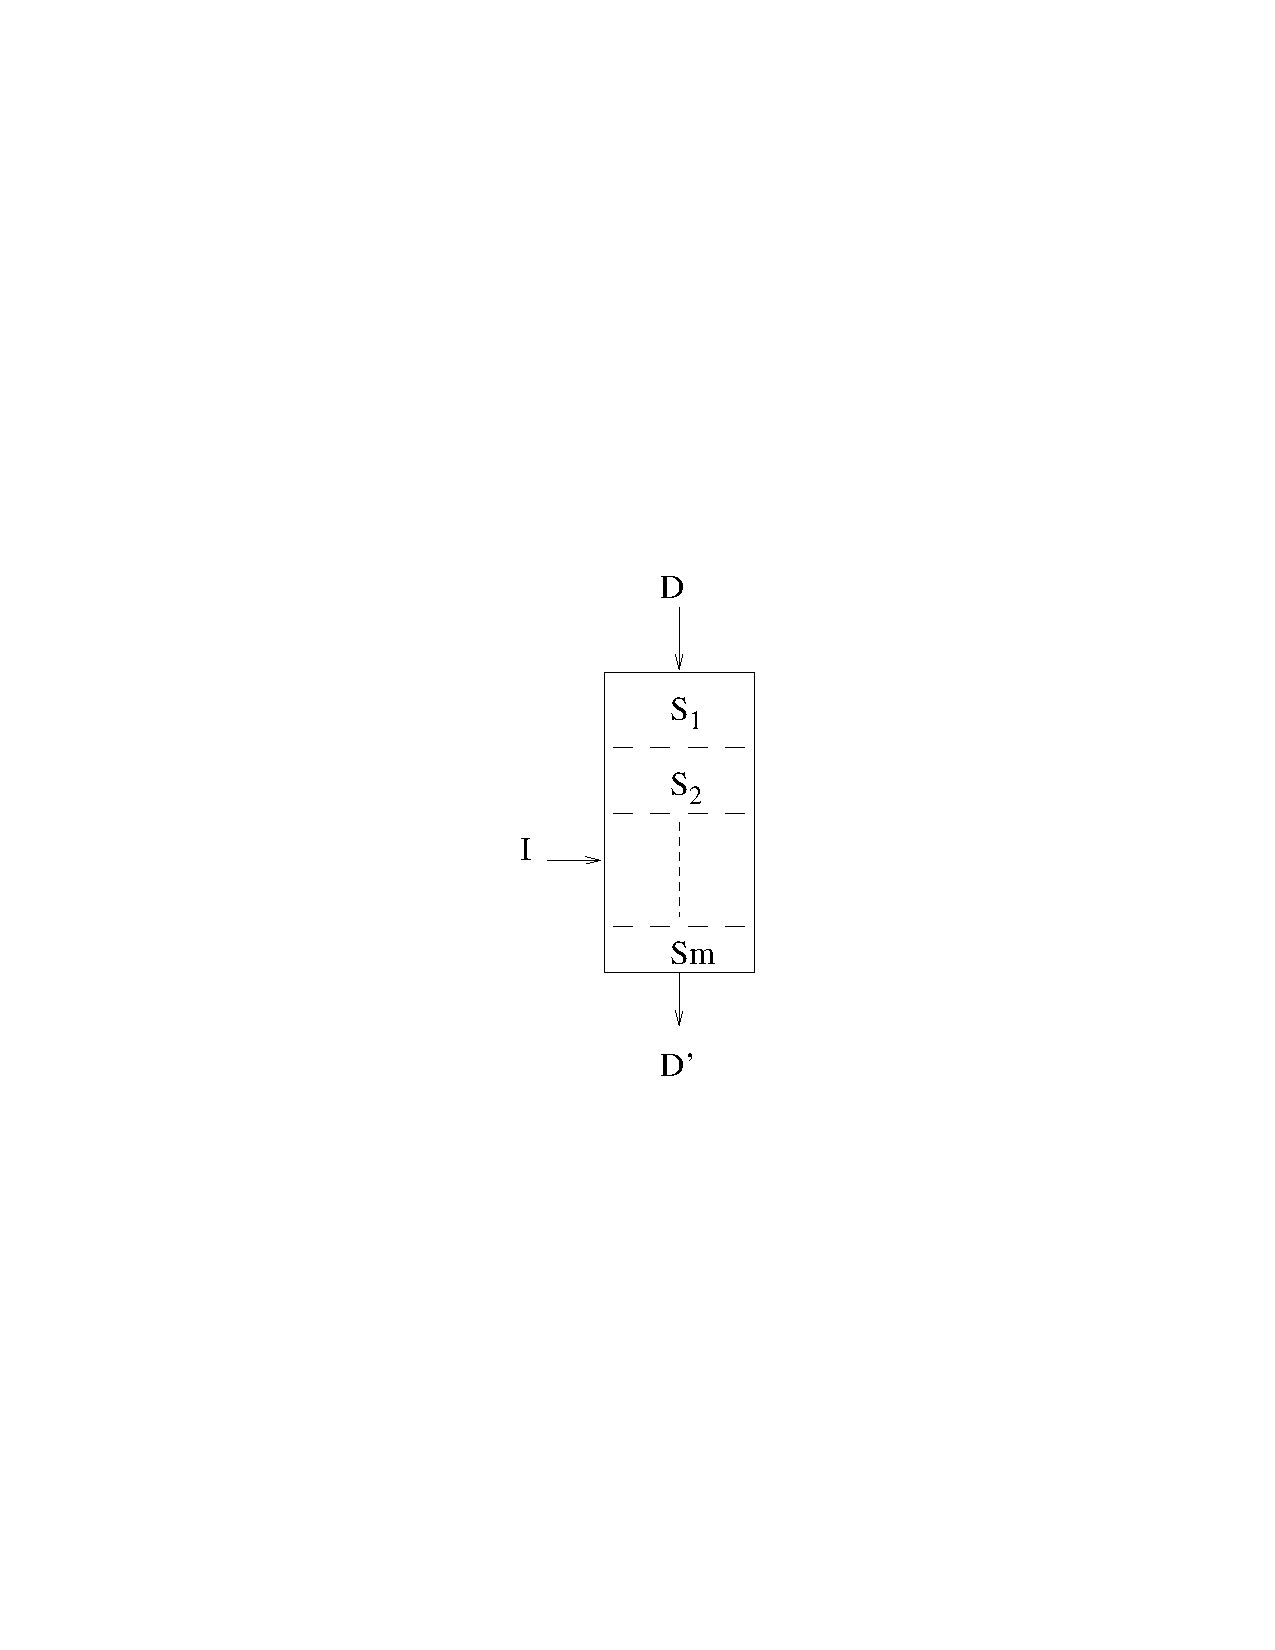
\includegraphics{fig1.pdf}} \par}
\caption{SISD Organization}
\end{figure}

2.{\bf{Single Instruction Stream Multiple Data Stream (SIMD):}} $m_{I}$ = 1, $m_{D}$ > 1. This category includes machines with a single program control
unit and multiple execution units. It also includes associative or content addressable memory processors. In such machines many stored data items may be
accessed and processed simultaneously. This is shown in fig 2.2. SIMD machines [2,9,10]permit explicit expression of parallelism in a program. Program segments
that
cannot be converted into parallel executable form are sent to the processing units and executed synchronously on data fetched from parallel memory modules
under the control of the control unit. An example of SIMD architecture is MasPar MP-2. While SIMD architectures work well for some applications, they don't
provide high performance across all applications and are viewed by many as specialty hardware.
\subsection{Vector Processors}
A subclass of the SIMD systems are vector processors[2,10]. Vector processors act on array of similar data rather than on single data items using specially
structured CPUs. When data can be manipulated by these vector units, results can be delivered with the rate of one, two, and in special cases three per clock
cycle. So, vector processors execute on their data in an almost parallel way but only when executing in vector mode. In this case they are several times
faster than when executing in conventional scalar mode. For practical purposes vector processors are therefore mostly regarded as SIMD machines.

\begin{figure}[ht]
{\centering \resizebox*{4in}{3in}{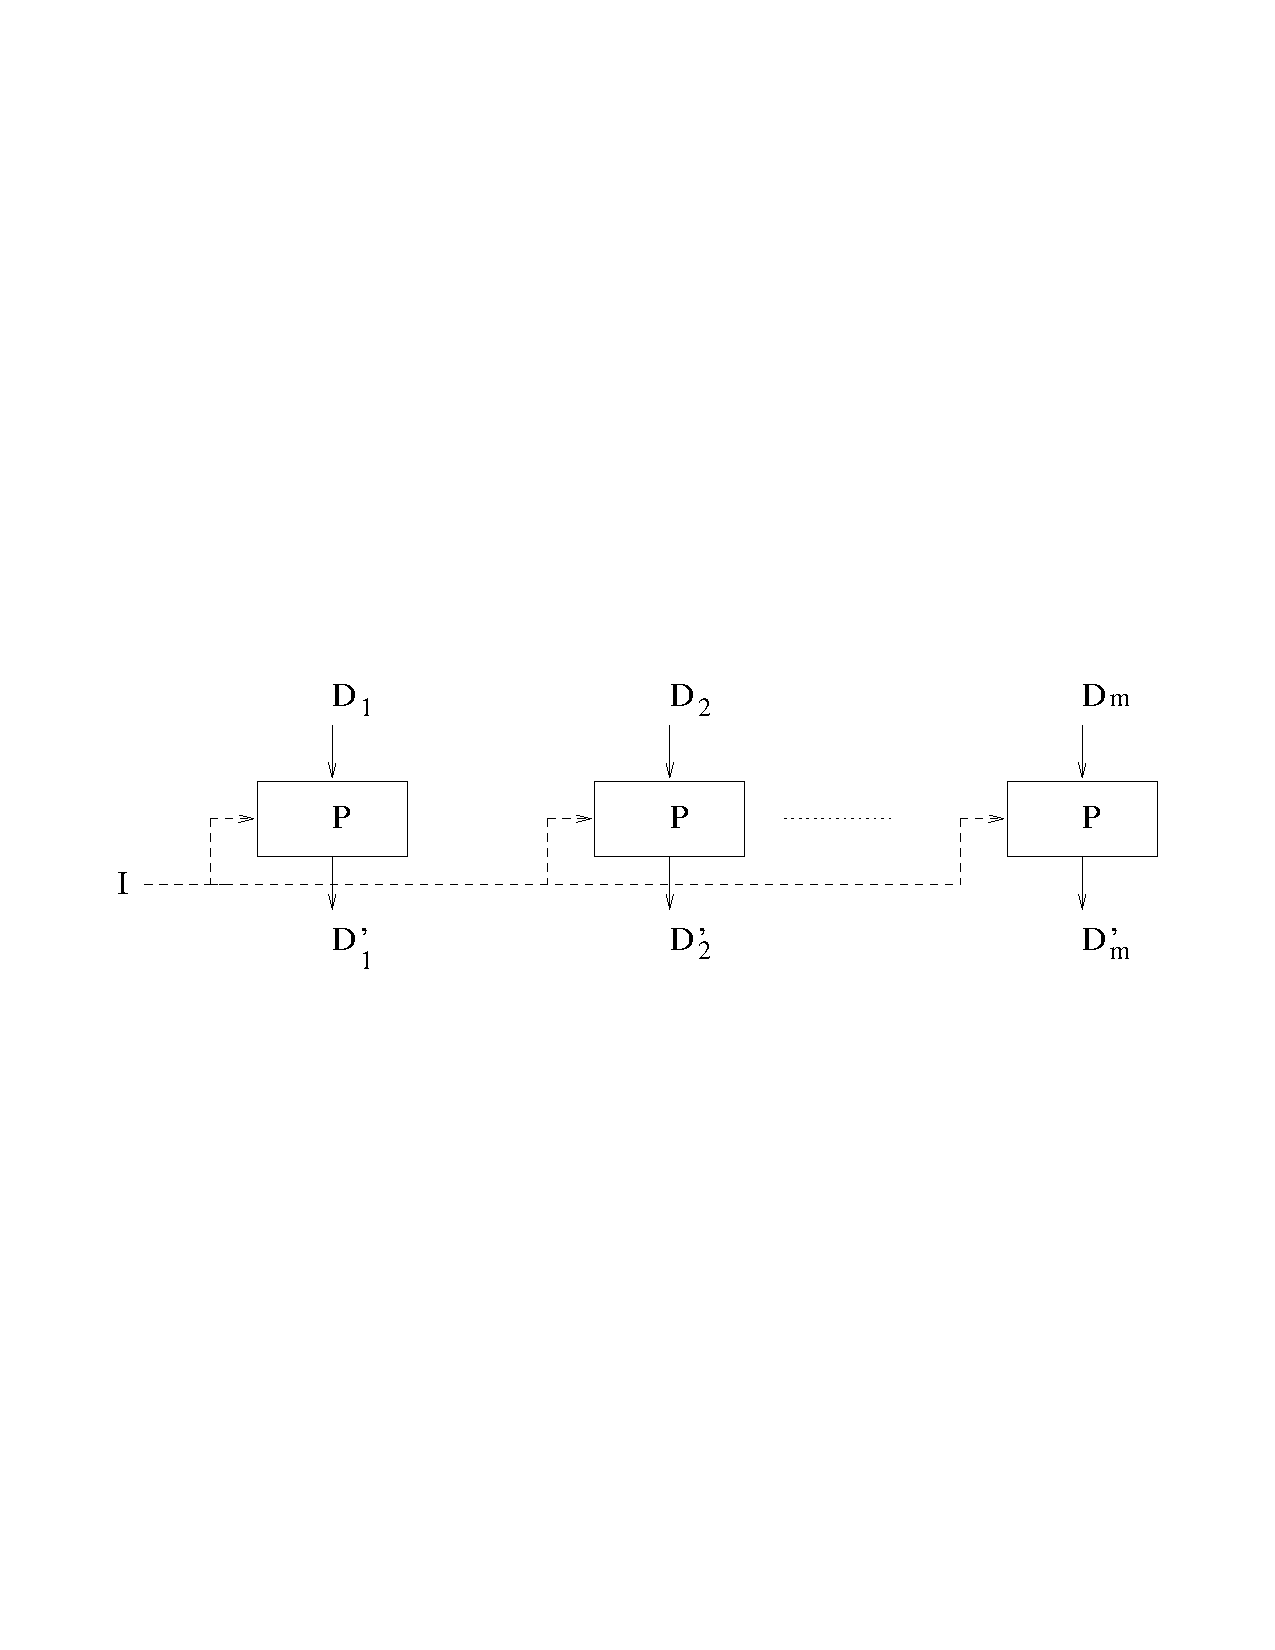
\includegraphics{fig4.pdf}} \par}
\caption{SIMD Organization}
\end{figure}
%\clearpage

3. {\bf{ Multiple Instruction Stream Single Data Stream (MISD):}} $m_{I}$ > 1, $m_{D}$ = 1. The class of machines that can be placed in this category seems
to be small. Pipeline processors may be considered to be MISD machines if the viewpoint is taken that each data item is processed by different instructions
in different segments of a pipeline. This is shown in fig 2.3.

\begin{figure}[ht]
{\centering \resizebox*{3.5in}{2.6in}{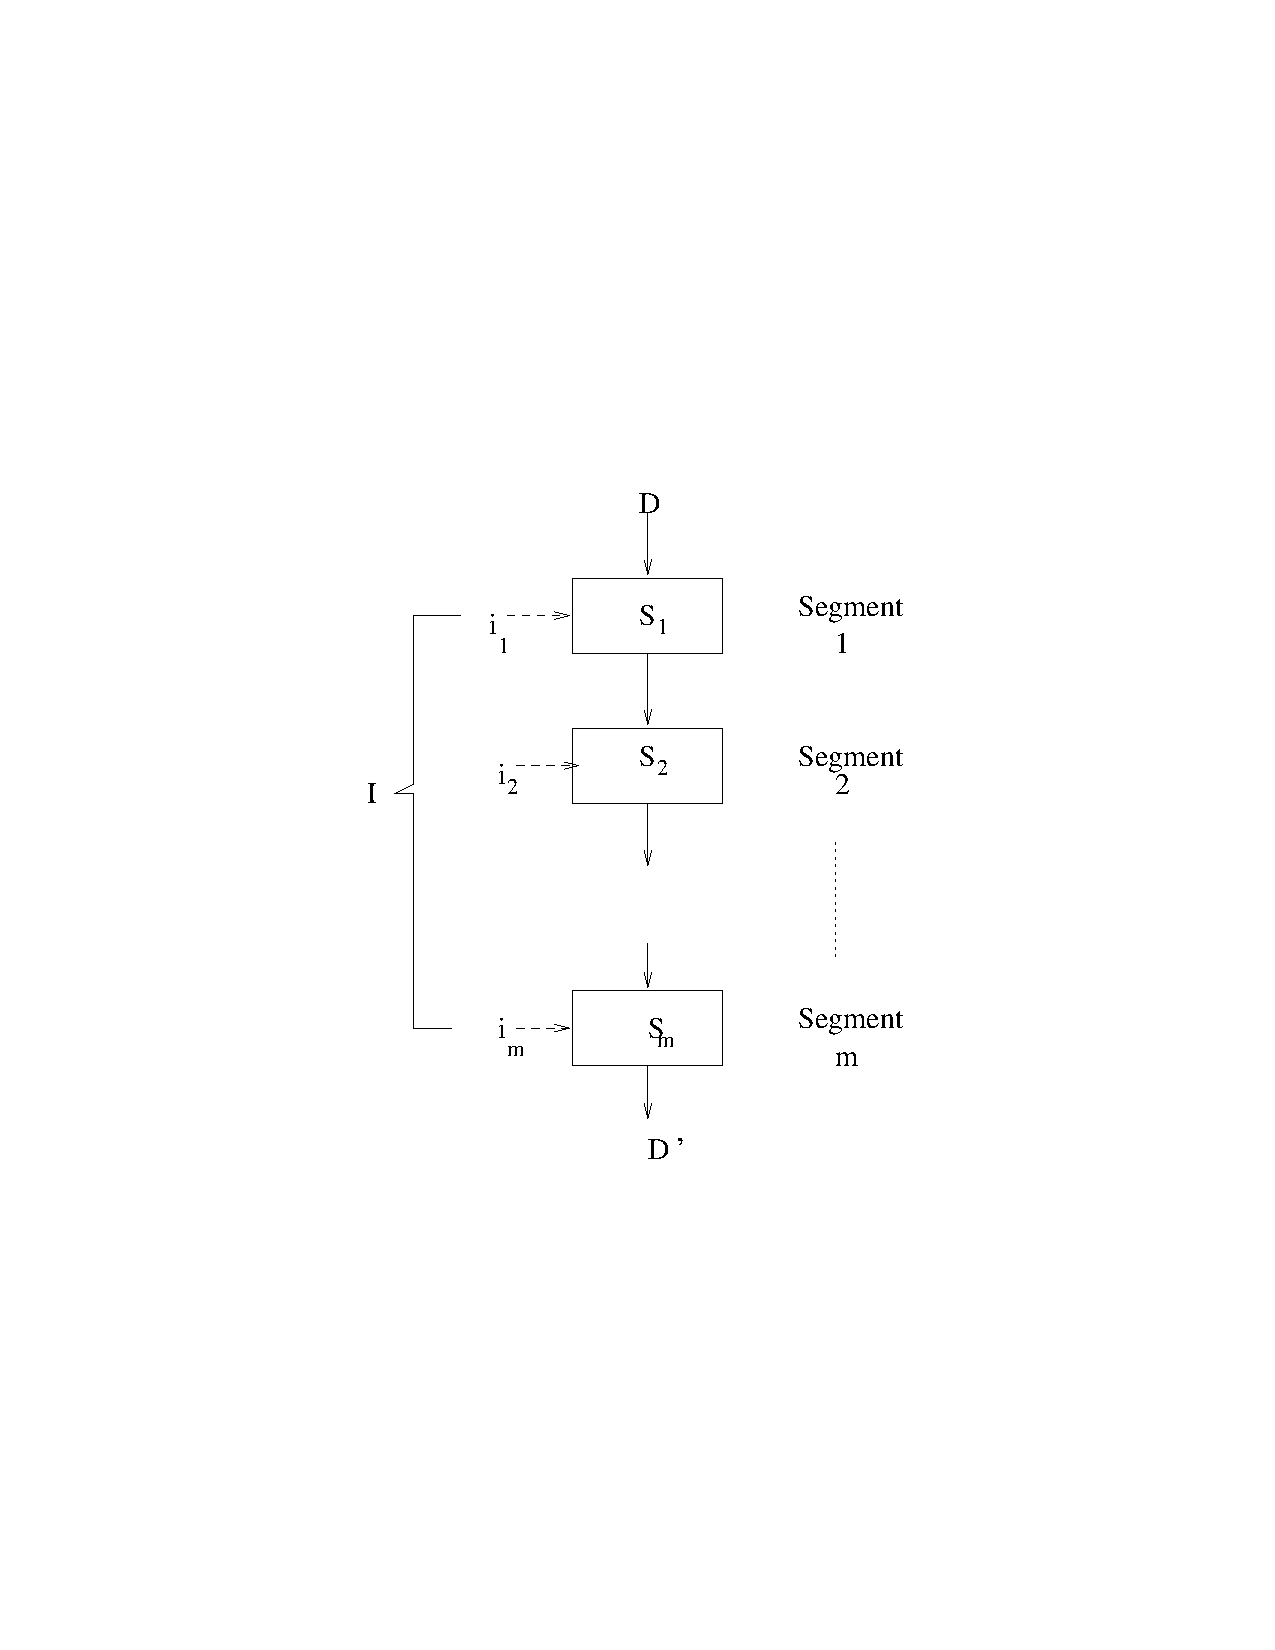
\includegraphics{fig7.pdf}} \par}
\caption{MISD Organization}
\end{figure}

4.{\bf{Multiple Instruction Stream Multiple Data Stream (MIMD):}} $m_{I}$ > 1, $m_{D}$ > 1. This class includes machines capable of executing several
independent programs simultaneously. The class of MIMD machines appears to coincide with the class of multiprocessors. This is shown in fig 2.4. Efficient
partitioning and assignments are essential for efficient multiprocessing. Most multiprocessor systems can be classified in this category. 

\begin{figure}[ht]
{\centering \resizebox*{4.2in}{2.9in}{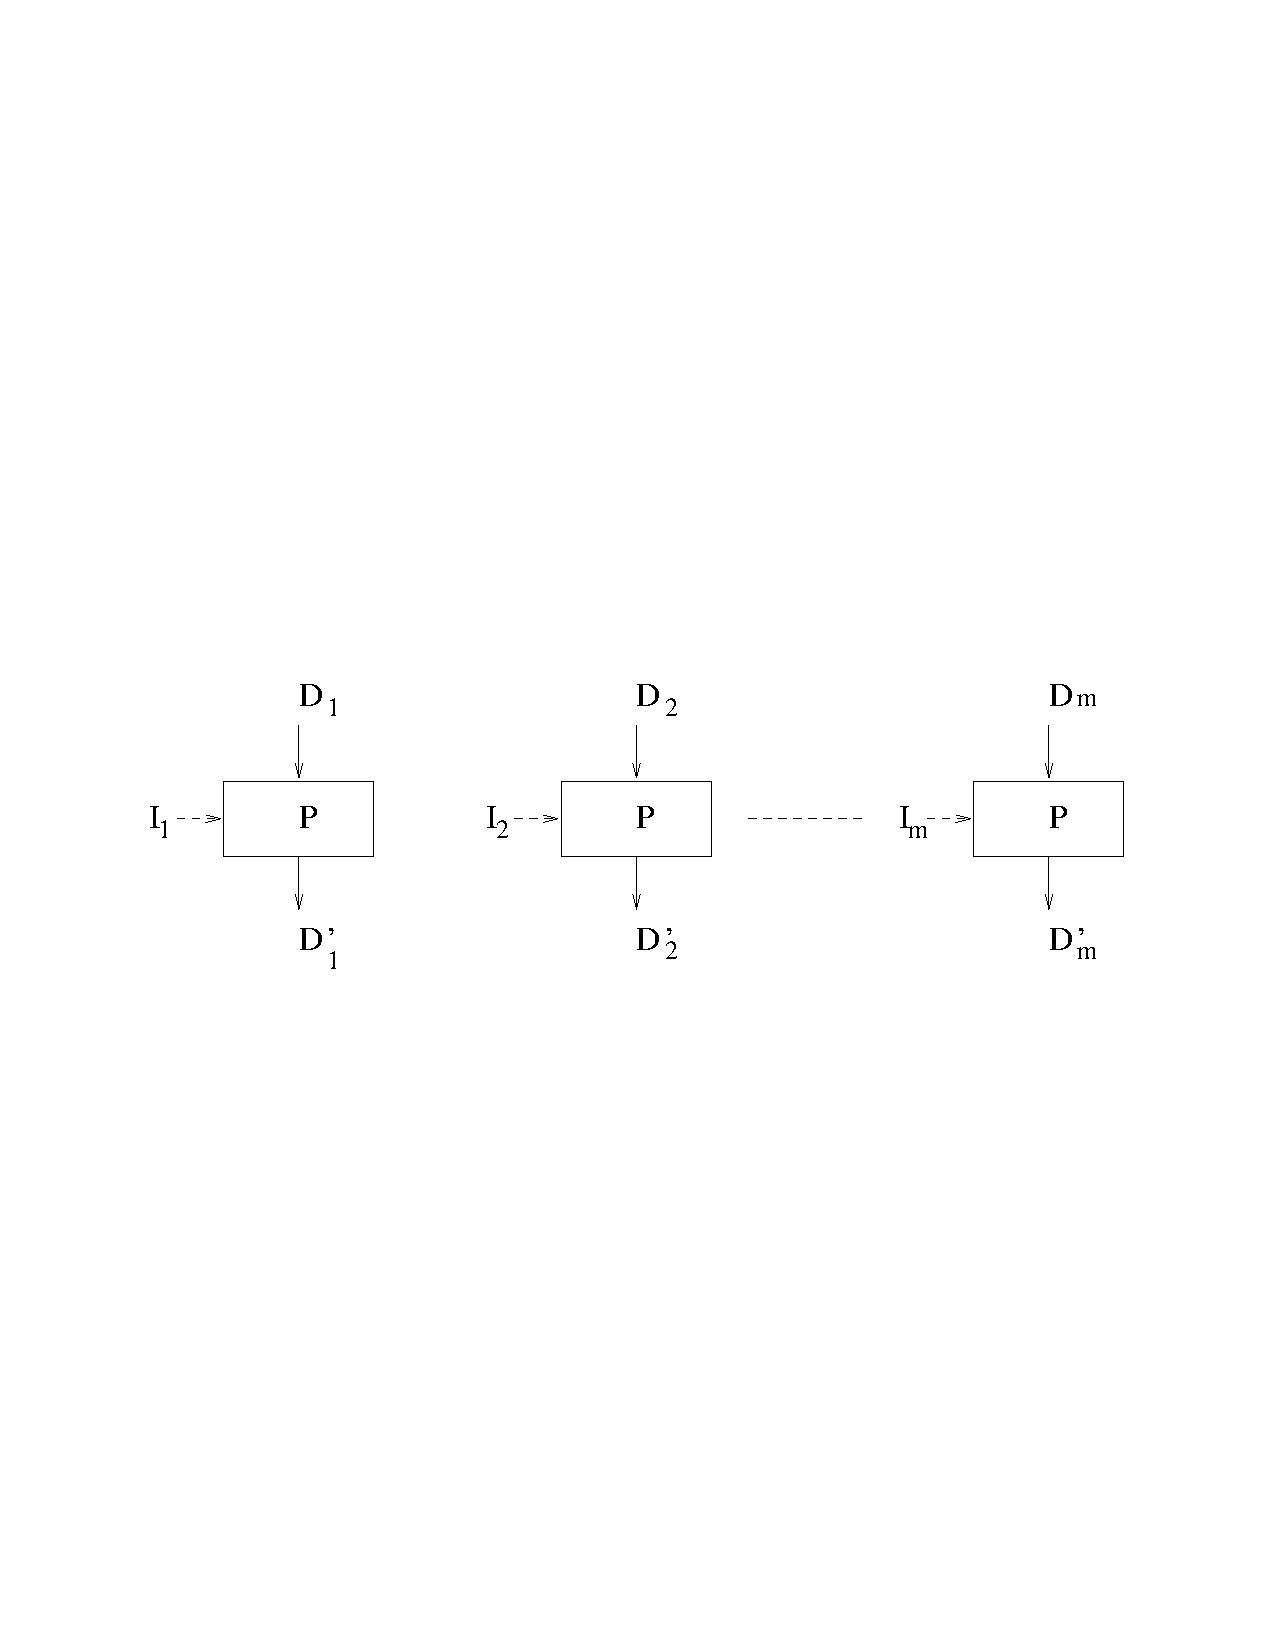
\includegraphics{fig3.pdf}} \par}
\caption{MIMD organization}
\end{figure}

\section{Parallelism within a single processor}
There are different ways to exploit parallelism with in a processor. Some of them are described below.
\subsection{Multiple functional units}
Early computers had three basic units: the main memory, the central processing unit (CPU), and the I/O subsystems. The operations were performed one function
per cycle. One of the first approaches to exploiting parallelism involved splitting up the functions of ALU, having different units for the different
operations and having the units operate in parallel. In order to take the advantage of the multiple functional units, the compiler had to be able to schedule
operations across the multiple functional units to keep the hardware busy.

\subsection{Pipelining}
A Pipeline[2,9,10] consists of a sequences of processing circuits, called segments, through which a data stream passes. Partial processing is
performed by each segment, and a final result is obtained after the data has passed through all segments of the pipeline. Occasionally it may be necessary to
make several passes through the pipeline in order to process a data set completely. Parallel processing is achieved by having distinct operands sets or
process in several segments at the same time. Each operand set moves from segment to segment until it has been completely processed.\par
\hspace{1in}Let $P_{1}$ be a non pipelined processor with total delay $t_{1}$, that is, with bandwidth $t_{1}^{-1}$. Let $P_{m}$ be an m-segment pipeline
version of $P_{1}$, in which each processing circuit $C_{i}$ has the same delay $t_{C}$ and $t_{R}$ is the same delay of each segment attributable to the
buffer register $R_{i}$ and its associated control logic. The total  delay of one segment of $P_{m}$ is $t_{C} + t_{R}$; hence the maximum throughput of
$P_{m}$ is $(t_{C} + t_{R})^{-1}$. Now if $P_{m}$ is formed by partitioning $P_{1}$ into segments of approximately same delay, then $t_{1} \approx mt_{C}$.
Hence the maximum throughput of $P_{1}$ is approximately $(mt_{C})^{-1}$. We conclude that $P_{m}$ has greater maximum throughput than $P_{1}$ if the following
condition is satisfied:
\begin{equation}
mt_{C} > t_{C} + t_{R}
\end{equation}
There are two areas where pipelining appears to be particularly appropriate:\par
\begin{itemize}
\item The transfer of instructions through the various stages in the instruction cycle of a CPU, which amounts to realizing most or all of the CPU in the form
of the pipeline called an Instruction Pipeline. The purpose of the instruction pipeline is to overlap some or all of the steps in the instruction cycle.
\item The implementation of the arithmetic operations particularly the more complex arithmetic operations such as those involving floating point numbers, a
      pipeline processor for this purpose is called an Arithmetic Pipeline.
\end{itemize}
In the Pipeline Processors [2,9,10], pipeline scheduling takes place which allows tasks to perform without collision. The execution of the pipelined
instruction incurs an overhead for filling the pipeline. Once the pipeline is filled, a result appears every clock cycle. The overhead or startup for such an
operations depends on the number of stages or segments.

\subsection{Overlapping} Some architectures allow for the overlap of operations if the two operations can be executed by the independent functional units.
Overlap is similar but not identical to pipelining. Both employ the subfunction partitioning, but in a slightly different manner. 

\subsection{RISC}
A RISC (Reduced Instruction Set Computer) is simpler in design and provides instruction execution at the rate of the one per clock cycle. RISC machines are
often associated with pipeline implementations since pipeline techniques are natural for achieving the goals of one instruction executed per machine
cycle.\par
\hspace{2in} There are many others architectures (e.g. VLIW) and techniques e.g. use of vector instructions, chaining, stripmining etc, used to gain the
performance within a microprocessor. With these, other issues like memory organisation (in practice use of cache, main memory), data organisation,
memory management came in picture and various ways have been found out and the development are still in progress. An example of how memory management
should be done, is given in subsection 2.4.1.

\section{Multi unit Processor}
A multi-unit processor [2,9,10] consists of a set of m disjoint processing elements each of which is capable of acting on a data stream independently of the
others. A central component of any multi unit processor system is a scheduler or control unit which coordinates activities among the various units. The
scheduler must preserve the precedence among the processes being executed and the available processing units as efficiently as possible. It must keep track
of the status(busy or idle) of each processing unit as well as any facilities such as registers or buses shared among them. This is actually done by
associating a status bit or flag with each processing unit and shared facility. Shared memory processors come in this category. These processors are based 
on the MIMD organisation.\par
\hspace{1in}For a programming standpoint it would be attractive if a distributed memory parallel computer would allow each process to treat all of the
memory in the system as a single large pool rather than separate distributed memories. This would
allow the programmer to reference data not locally contained through a conventional assignment or reference rather than calls to the message passing library.
This would give the illusion of shared memory in a system that has physically distributed memory. Underneath the programming layer there would be separate
memories that the system would manage. This would free the programmer from writing explicit message passing statements. This type of organisation is called
Virtual Shared Memory. It blurs the distinction between traditional shared memory MIMD and traditional distributed memory MIMD computing. In this memory
organisation, to ensure performance, minimizing memory transfers is still critical.


\section{System Requirements}
A computer using parallel processors to achieve very high throughput poses a number of special design  problems. Chief among these is that of moving
instructions and data to and from the processors at or near their streaming modes. A possible solution is to partition main memory into independently
addressable modules or banks so that words can be accessed simultaneously. Instructions and operands addresses should be distributed uniformly among the
memory modules, so that successive access are made to different memory modules; this is called address interleaving. A communication of high bandwidth is
also needed between the memory banks and the processors. \par
\hspace{1in} Just as instructions and data are carefully distributed among the memory modules, they must also be carefully distributed to the various
processing elements. This requires the program control unit to schedule the tasks performed by the processing elements to minimize the number of conflicts
and idle processors.

\subsection{Memory Issues}
A basic problem in all parallel processors with a shared main memory [1,2,10] is that of moving data and instructions between the processors and main memory at
sufficiently high rates to maintain the system performance close to its maximum level. One common solution is to partition the memory into multiple modules or
memory banks with address interleaving. The individual memory modules can be accessed in parallel, thereby increasing the system's effective memory bandwidth.
The data and instruction address must be distributed in a balanced fashion among the available memory modules by the system software, and special hardware is
needed to control access to the memory modules. \par
\hspace{1in} In many computer systems, large programs often cannot fit into the main memory for execution. Even if there is enough main memory for a program,
the main memory may be shared between a number of users, causing any one program to occupy only a fraction of memory, which may not be sufficient for the
program to execute. The usual solution is to introduce management schemes that intelligently allocate portions of memory to users as necessary for the
efficient running of their programs. The goal of designing a multilevel memory hierarchy is to achieve a performance close to that of the fastest memory, at a
cost per bit to that of the slowest memory. In earlier computers a technique called overlays was used, but more common today is the use of virtual memory,
in which data is organized as pages and whenever a request is made, page is transfered from virtual memory to main memory, main memory to cache memory and then
from cache memory to the registers inside the CPU. Performance of the computer also depends on the numbers of page faults or the number of times the data
transfer takes place. Though the virtual memory management is done by the operating system and the user has no information about the pages that are
actually in main memory, he can influence the number of large faults. \par
\hspace{1in} The example itself concerns the dense matrix-matrix multiplication [7,8] $C = AB + C$. The matrices are square and of order 1024. Assume a page
contains 65,536 elements; then it follows that 64 columns of a matrix can be stored on 1 page and that all three matrices can be stored on 48 pages in total.
Let us assume that the available main memory space can contain 16 pages. This implies that if we have access to successive columns of a matrix, we have a page
fault after every 64 columns. Here it is also assumed that a page fault takes about 0.5 seconds of I/O time. Different ways to compute $C = AB + C$ are given
below:

\subsubsection{Inner-product approach - ijk}
\begin{verbatim}
	DO 30 I = 1, N
	   DO 20 J = 1, N
	      DO 10 K = 1, N
                 C(I,J) = A(I,K) * B(K,J) + C(I,J) 
  10          CONTINUE
  20       CONTINUE
  30    CONTINUE
\end{verbatim}

This scheme leads to paging A 1024*16*1024 times. Thus, a total number of about 16 million page faults results in a minimal I/O time of at least 93 days, and
in reality the turn around time will be considerably larger since the machine usually has other works.

\subsubsection{Column-wise update of C - jki}

\begin{verbatim}

        DO 30 J = 1, N
           DO 20 K = 1, N
              DO 10 I = 1, N
                C(I,J) = A(I,K) * B(K,J) + C(I,J)
  10          CONTINUE
  20       CONTINUE
  30    CONTINUE

\end{verbatim}

This scheme leads to paging A 1024*16 times, B and C only 16 times. Thus, total number of about 16,000 page faults results in a minimal I/O time of
about 2.25 hours.


\subsubsection{Partitioning the matrices into block-columns - blocked jki}

\begin{verbatim}

        DO 40 J = 1, N, NB
           DO 30 K = 1, N, NB
              DO 20 JJ = J, J+NB-1
                 DO 10 KK = K, K+NB-1
                C(:, JJ) = A(:, KK) * B(KK, JJ) + C(:, JJ)
  10             CONTINUE
  20          CONTINUE
  30       CONTINUE
  40    CONTINUE

\end{verbatim}

The great gain is made with respect to the I/O time: the scheme leads to paging A 4 times and B and C only once, resulting in only 96 page faults, and hence
takes only a modest 70 seconds of I/O time.



\subsection{Interconnection Issues}
A parallel computer's interconnection network [10] plays a major role in determining its performance. Static interconnection structures such as trees are best
suited to the execution of algorithm that requires infrequent processor communication (to share results or intermediate results etc.) and to confine most
communication to neighbour processors. From the physical standpoint a network consists of a number of switching elements and interconnection links. The two
major switching methodologies are circuit switching (suitable for bulk data transfer) and packet switching (suitable for short data transfer). There is one
more system which is the hybrid of these two. Communication links are divided into two groups, regular and irregular. Regular are again divided into two
categories: static ( one dimensional, two dimensional, three dimensional, and hypercube)  and dynamic (single-stage, multistage, and crossbar).

\section{Message Passing}
The message passing [10] programming model is based on the assumption that there are a number of processes in the system which have their local memories and
can communicate with each other by coordinating memory transfers from one process to another. Thus, this model is of primary importance for distributed memory
parallel computers. On the shared memory computers, communication between tasks executing on different processors is usually through shared data or
by means of semaphores, variables used to control access to shared data. On a local-memory machine, however, communication is more explicit and is
normally done through message passing. \par
\hspace{1in} In message passing, data is passed between processors by a single send and receive mechanism [3,10]. The main variants are whether an
acknowledgement is returned to the sender, whether receiver is waiting for the message, and whether either processor can continue with other computations while
the message is
being sent. An important feature of message passing is that, on nearly all machines, it is much more costly than floating point arithmetic. Message passing
performance is usually measured in units of time or bandwidth (bytes per second). For short messages, time is used as performance unit and for long messages
bandwidth is used as a measure. \par
\hspace{1in} There are a number of factors that can affect message passing performance. The number of times the message has to be copied or touched (e.g.
checksums) is probably the most influential effect on the message passing. Second order effects of message size may also affect performance. For small
messages context switch times also contribute to delays. The other parameters, which affect the performance of the message passing, are
aggregate bandwidth of the network, the amount of concurrency, reliability, scalability, and congestion management.\par
\hspace{1in} To enhance the development of parallel application some standard interface for parallel computing has been developed over years. Out of them
MPI, PVM, and HPF are the foremost. The Message Passing Interface (MPI) [10] is a portable message passing standard that facilitates the developments of the
parallel application and libraries. The standard defines the syntax and semantics of core library routines useful to a wide range of users writing portable
message passing programs in Fortran, C, C++. MPI also forms a possible target for the compilers of languages such as High Performance Fortran. Commercial and
free, public domain implementations of MPI already exist. These run both on tightly coupled, massively parallel machines (MPPs) and on network of workstations
(NOWs). Parallel Virtual Machine or PVM [3] is used to provide an excellent platform for inter-processor communication and convert the distributed array of
processors into one virtual single processor. It is a software package that allows a heterogeneous or serial computer to appear as a
single concurrent computational resource. The individual computers may be shared- or local-memory multiprocessors, vector supercomputers, specialized graphics
engines, or scalar workstations, that may be interconnected by a variety of networks, such as Ethernet, FDDI. PVM consists of two parts: a daemon process that
any user can install on a machine and a user library that contains routines for initiating processes on other machines, for communicating between processes
and changing the configuration of machines. PVM is available on Internet site [4] and it is a freeware tool. \par

\section{Advantages of MultiProcessor System}
There are several reasons to build tightly coupled systems.

\begin{enumerate}
\item Increase in throughput.
\item Saving of money.
\item Increase in reliability
\end{enumerate}
\hspace{1in} The most common multiprocessor systems now use the {\em Symmetrical Multiprocessing Model}, in which each processor runs an ideal copy  of the
operating system, and these copies communicate with each other as needed. Some systems use {\em Asymmetrical Multiprocessing Model}, in which each processor
is assigned a specific task. A master processor controls the system; the other processors either look to the master for instruction or have predefined tasks. 
This scheme defines a master-slave relationship. The master processor schedules and allocates work to the slave processors.\par
\hspace{1in} There is also a variety of reasons for building distributed systems, the major ones being these:
\begin{enumerate}
\item Resource sharing
\item Computation speedup
\item Reliability
\item Communication
\end{enumerate} 
 
